% 帐号与密码

\section {帐号与密码}

    帐号是在网络和多用户操作系统中保存着一种记录,用于记录授权用户的行为。网络帐户由网络管理员创建,用来验证用户和管理与每个用户相关的策略,例如访问权限。账号是数字时代的代表,就是每个人在特定的项目中所代表自己的一些数字等。账号有时可以由中文或英文组成,甚至是一些符号。 在多数场合下会被误写作“帐号”

\subsection {帐号密码的重要性}

    密码是安全基础的核心。如果危及到密码,那个基本的安全机制和模式将遭到严重影响。

    \begin{center}
        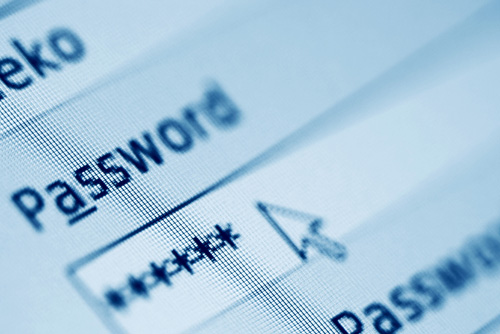
\includegraphics[scale=.6] {password.jpg}
    \end{center}

    一个强固的密码至于要有下列四方面内容的三种:

    \begin{itemize}
        \item 大写字母
        \item 小写字母
        \item 数字
        \item 非字母数字的字符,如标点符号
    \end{itemize}

    强固的密码还要符合下列的规则

    \begin{itemize}
        \item 不使用普通的名字或昵称
        \item 不使用普通的个人信息,如生日日期
        \item 密码里不含有重复的字母或数字
        \item 至少使用八个字符
    \end{itemize}

    从黑客的思想考虑,避免密码容易被猜出或发现(比如不要写到纸条上放到抽屉里)。

    总的来说,个人密码安全需要遵循如下几个简单的要求:对于不同的网络系统使用不同的密码,对于重要的系统使用更为安全的密码。绝对不要所有系统使用同一个密码。对于那些偶尔登录的论坛,可以设置简单的密码;对于重要的信息、电子邮件、网上银行之类,必需设置为复杂的密码。永远也不要把论坛、电子邮箱和银行账户设置成同一个密码。

\subsection {密码分类}

    处于安全考虑,最好将自己的常用密码分类:弱密码、中密码、强密码

    \begin{enumerate}
        \item 弱密码

        最容易记忆的,且默认是可以丢失的密码。

        各类中小网站、论坛、社区、个人网站等使用。

        原因:这些网站的安全性可能都不太好,有些只是将密码MD5一下存储,有些可能还会明文存储密码。黑客很容易从这些网站盗窃用户的密码。

        \item 中密码

        中等强度密码,8个字符以上,有一定抗穷举能力的。

        中等密码主要在国内门户网站、大型网站、门户微博、社交网站等使用,但不要在主要邮箱里使用。门户网站最好绑定手机号码。

        原因:大网站的安全性较好,通常被破解的可能性低,在大网站使用的密码要强度可以稍强。

        需要注意的是,有些门户网站(例如新浪、搜狐等)即提供微博,又提供邮件系统,如果系统默认建立了这些邮箱,那建议不要在任何地方使用这些邮箱,如果要使用邮箱,最好确认该邮箱具有独立密码功能。

        其中有一个例外是腾讯邮箱,腾讯邮箱支持邮箱的单独密码,设置好了以后,用户需要输入QQ密码和邮箱密码两个之后才能使用。

        所有游戏帐号使用单独的密码。

        \item 强密码

        强密码要求至少8个字符以上,不包含用户名、真实姓名或公司名称,不包含完整的单词,包含字母、数字、特殊符号在内。

        强密码主要用于邮箱、网银、支付系统等。

        这类网站是最核心最重要的网站,网银涉及到用户的财产安全,邮箱则可以重置用户所有注册过的网站密码,因此这类网站一定要用强密码,保证其绝对安全性。

        密码穷举对于简单的长度较少的密码非常有效,但是如果网络用户把密码设的较长一些而且没有明显规律特征(如用一些特殊字符和数字字母组合),那么穷举破解工具的破解过程就变得非常困难,破解者往往会对长时间的穷举失去耐性。通常认为,密码长度应该大于8位,密码中最好包含字母数字和符号,不要使用纯数字的密码,不要使用常用英文单词的组合,不要使用自己的姓名做密码,不要使用生日做密码。
    \end{enumerate}


% 基于角色的访问控制

\section {基于角色的访问控制}

    \semsys 在访问安全控制中使用基于 RBAC 的模型来管理。 基于角色的访问控制(Role-Based Access Control)作为传统访问控制(自主访问,强制访问)的有前景的代替受到广泛的关注。在RBAC中,权限与角色相关联,用户通过成为适当角色的成员而得到这些角色的权限。这就极大地简化了权限的管理。在一个组织中,角色是为了完成各种工作而创造,用户则依据它的责任和资格来被指派相应的角色,用户可以很容易地从一个角色被指派到另一个角色。角色可依新的需求和系统的合并而赋予新的权限,而权限也可根据需要而从某角色中回收。角色与角色的关系可以建立起来以囊括更广泛的客观情况。

\subsection {RBAC简介}

    RBAC支持三个著名的安全原则:最小权限原则,责任分离原则和数据抽象原则。最小权限原则之所以被RBAC所支持,是因为RBAC可以将其角色配置成其完成任务所需要的最小的权限集。责任分离原则可以通过调用相互独立互斥的角色来共同完成敏感的任务而体现,比如要求一个计帐员和财务管理员共参与同一过帐。数据抽象可以通过权限的抽象来体现,如财务操作用借款、存款等抽象权限,而不用操作系统提供的典型的读、写、执行权限。然而这些原则必须通过RBAC各部件的详细配置才能得以体现。

    RBAC有许多部件,这使得RBAC的管理多面化。尤其是,我们要分割这些问题来讨论:用户与角色的指派;角色与权限的指派;为定义角色的继承进行的角色与角色的指派。这些活动都要求把用户和权限联系起来。然而在很多情况下它们最好由不同的管理员或管理角色来做。对角色指派权限是典型的应用管理者的职责。银行应用中,把借款、存款操作权限指派给出纳角色,把批准贷款操作权限指派给经理角色。而将具体人员指派给相应的出纳角色和管理者角色是人事管理的范畴。角色与角色的指派包含用户与角色的指派、角色与权限的指派的一些特点。更一般来说,角色与角色的关系体现了更广泛的策略。

\subsection {RBAC基本概念}

    RBAC认为权限授权实际上是Who、What、How的问题。在RBAC模型中,who、what、how构成了访问权限三元组,也就是“Who对What(Which)进行How的操作”。

    \begin{itemize}
        \item Who:权限的拥用者或主体(如Principal、User、Group、Role、Actor等等)
        \item What:权限针对的对象或资源(Resource、Class)。
        \item How:具体的权限(Privilege,正向授权与负向授权)。
        \item Operator:操作。表明对What的How操作。也就是Privilege+Resource
        \item Role:角色,一定数量的权限的集合。权限分配的单位与载体,目的是隔离User与Privilege的逻辑关系.
        \item Group:用户组,权限分配的单位与载体。权限不考虑分配给特定的用户而给组。组可以包括组(以实现权限的继承),也可以包含用户,组内用户继承组的权限。User与Group是多对多的关系。Group可以层次化,以满足不同层级权限控制的要求。
    \end{itemize}

    RBAC的关注点在于Role和User, Permission的关系。称为User assignment(UA)和Permission assignment(PA).关系的左右两边都是Many-to-Many关系。就是user可以有多个role,role可以包括多个user。

    凡是用过RDBMS都知道,n:m 的关系需要一个中间表来保存两个表的关系。这UA和PA就相当于中间表。事实上,整个RBAC都是基于关系模型。

    Session在RBAC中是比较隐晦的一个元素。标准上说:每个Session是一个映射,一个用户到多个role的映射。当一个用户激活他所有角色的一个子集的时候,建立一个session。每个Session和单个的user关联,并且每个User可以关联到一或多个Session.

    在RBAC系统中,User实际上是在扮演角色(Role),可以用Actor来取代User,这个想法来自于Business Modeling With UML一书Actor-Role模式。考虑到多人可以有相同权限,RBAC引入了Group的概念。Group同样也看作是Actor。而User的概念就具象到一个人。

    这里的Group和GBAC(Group-Based Access Control)中的Group(组)不同。GBAC多用于操作系统中。其中的Group直接和权限相关联,实际上RBAC也借鉴了一些GBAC的概念。

    Group和User都和组织机构有关,但不是组织机构。二者在概念上是不同的。组织机构是物理存在的公司结构的抽象模型,包括部门,人,职位等等,而权限模型是对抽象概念描述。组织结构一般用Martin fowler的Party或责任模式来建模。

    Party模式中的Person和User的关系,是每个Person可以对应到一个User,但可能不是所有的User都有对应的Person。Party中的部门Department或组织Organization,都可以对应到Group。反之Group未必对应一个实际的机构。例如,可以有副经理这个Group,这是多人有相同职责。

    引入Group这个概念,除了用来解决多人相同角色问题外,还用以解决组织机构的另一种授权问题:例如,A部门的新闻我希望所有的A部门的人都能看。有了这样一个A部门对应的Group,就可直接授权给这个Group。


\subsection {RBAC的许可配置}

      基于角色访问控制的要素包括用户、角色、许可等基本定义。

    在RBAC中,用户就是一个可以独立访问计算机系统中的数据或者用数据表示的其他资源的主体。角色是指一个组织或任务中的工作或者位置,它代表了一种权利、资格和责任。许可(特权)就是允许对一个或多个客体执行的操作。一个用户可经授权而拥有多个角色,一个角色可由多个用户构成;每个角色可拥有多种许可,每个许可也可授权给多个不同的角色。每个操作可施加于多个客体(受控对象),每个客体也可以接受多个操作。

    \begin{figure}
        \centering
        \begin{tikzpicture}[
                node distance=6em,
                op/.style={draw, ellipse}
                ]
            \node[op] (user) {用户};
            \node[op, right of=user] (role) {角色};
            \node[op, right of=role] (oper) {操作};
            \node[op, right of=oper] (entity) {客体};
            \draw[latex-latex] (user) -- (role);
            \draw[latex-latex] (role) -- (oper);
            \draw[latex-latex] (oper) -- (entity);
            \node[draw, circle, fit=(oper) (entity)] (outl) {};
            \node[below=2mm of outl.north] {许可};
        \end{tikzpicture}
        \caption {许可配置说明} \label{fig:permConfig1}
    \end{figure}

    用户表(USERS)包括用户标识、用户姓名、用户登录密码。用户表是系统中的个体用户集,随用户的添加与删除动态变化。

    角色表(ROLES)包括角色标识、角色名称、角色基数、角色可用标识。角色表是系统角色集,由系统管理员定义角色。

    客体表(OBJECTS)包括对象标识、对象名称。客体表是系统中所有受控对象的集合。

    操作算子表(OPERATIONS)包括操作标识、操作算子名称。系统中所有受控对象的操作算子构成操作算子表。

    许可表(PERMISSIONS)包括许可标识、许可名称、受控对象、操作标识。许可表给出了受控对象与操作算子的对应关系。

    角色/许可授权表包括角色标识、许可标识。系统管理员通过为角色分配或取消许可管理角色/许可授权表。

    RBAC的基本思想是:授权给用户的访问权限,通常由用户在一个组织中担当的角色来确定。RBAC中许可被授权给角色,角色被授权给用户,用户不直接与许可关联。RBAC对访问权限的授权由管理员统一管理,RBAC根据用户在组织内所处的角色作出访问授权与控制,授权规定是强加给用户的,用户不能自主地将访问权限传给他人,这是一种非自主型集中式访问控制方式。例如,在医院里,医生这个角色可以开处方,但他无权将开处方的权力传给护士。

    在RBAC中,用户标识对于身份认证以及审计记录是十分有用的;但真正决定访问权限的是用户对应的角色标识。用户能够对一客体执行访问操作的必要条件是,该用户被授权了一定的角色,其中有一个在当前时刻处于活跃状态,而且这个角色对客体拥有相应的访问权限。即RBAC以角色作为访问控制的主体,用户以什么样的角色对资源进行访问,决定了用户可执行何种操作。

    ACL直接将主体和受控客体相联系,而RBAC在中间加入了角色,通过角色沟通主体与客体。分层的优点是当主体发生变化时,只需修改主体与角色之间的关联而不必修改角色与客体的关联。


\practices
\subsection{角色,组,用户之间的关系}
    模型图:
    \screenshot{role_group_user.png}
    \ol {
        \item  一个用户可以有很多角色
        \item  一个用户可以属于很多组
        \item  一个组可以拥有很多用户
        \item  一个组可以有很多角色
        \item  一个角色可以对应很多用户
        \item  一个角色可以对应很多组
        \item  组是一个树型的结构。一个组下面可以有很多组
        \item  角色是一个树型的结构。一个角色下面可以有很多角色
    }

\subsection{登录}
    \ol {
        \item  在浏览器地址栏输入本系统的网址
            登录界面如下图
            \screenshot{login.png}
        \item  输入用户名
        \item  输入密码
        \item  点击登录
    }
    登录后的界面如下:
    \screenshot{welcome.png}

\subsection{角色管理}
    对应菜单:选项$\rightarrow$系统$\rightarrow$安全主体$\rightarrow$角色管理
    \opset{角色管理}{
        \item \ops{新建角色}{
            \item  点击工具栏上的\button{新建}按钮,弹出新建用户角色对话框
                \screenshot{45.png}
            \item  (如果有上级角色)点击按钮,弹出选择上级角色对话框
                \screenshot{46.png}
            \item  选择上级角色,点击\button{确定}按钮,完成上级角色选择
            \item  (如果没有上级角色)点击\button{X按钮},删除上级角色
            \item  输入角色\textbox{代码}
            \item  输入角色\textbox{名称}
            \item  点击\button{保存}按钮,完成角色新建
        }
        \item \ops{编辑角色}{
            \item  选择需要修改的角色
            \item  点击工具栏上的\button{修改}按钮,弹出修改角色对话框
            \item  修改相应的内容,过程类似与新建角色
            \item  点击\button{保存}按钮,完成角色信息修改
        }
        \item  \ops{查看角色}{
            \item  选择需要查看的角色
            \item  点击工具栏上的\button{查看}按钮,查看角色的详细信息
        }
        \item  \ops{删除角色}{
            \item  点击\button{删除}按钮,弹出确认删除对话框
                \screenshot{47.png}
            \item  点击\button{确定}按钮,完成角色删除
        }
    }

\subsection{组管理}
    \opset{组管理}{
        \item  \ops{新建用户分组}{
            \item  点击\button{新建}按钮,弹出新建用户组对话框
                \screenshot{42.png}
            \item  点击按钮,弹出选择上级分组对话框
                \screenshot{43.png}
            \item  选择上级用户组,点击\button{确定}按钮,完成选择
            \item  如果不需要上级分组)点击\button{X按钮}删除
            \item  输入组的\textbox{代码}
            \item  输入组的\textbox{名称}
            \item  输入组的\textbox{描述}
            \item  点击\button{保存}按钮,完成新用户组的添加
        }
        \item  \ops{编辑用户分组}{
            \item  选择用户分组
            \item  点击工具栏上的\button{编辑}按钮,弹出编辑用户组对话框
            \item  编辑相关信息,过程类似于新建用户组
            \item  点击\button{保存}按钮,完成用户组编辑
        }
        \item  \ops{查看用户分组}{
            \item  选择需要查看的用户组
            \item  点击工具栏上的查看按钮,显示用户分组明细信息
        }
        \item  \ops{删除用户分组}{
            \item  点击工具栏上的\button{删除}按钮,弹出确认删除对话框
                \screenshot{44.png}
            \item  点击\button{确定}按钮,完成用户分组删除
        }
    }

\subsection{用户管理}
    \opset{用户管理}{
        \item  \ops{新建用户}{
            \item  点击工具栏上的\button{新建}按钮,弹出新建用户对话框
                \screenshot{48.png}
            \item  输入用户\textbox{代码},(注意:一经确定,不可跟改)
            \item  输入用户\textbox{名称}
            \item  输入用户\textbox{密码}
            \item  \textbf{确认密码}
            \item  点击\button{保存}按钮,完成用户添加
        }
        \item  \ops{查看用户}{
            \item --该功能被禁用
        }
        \item  \ops{编辑用户}{
            \item  选择用户
            \item  点击工具栏上的\button{修改}按钮,弹出修改用户信息对话框
            \item  修改相应内容(用户代码不能修改)
            \item  点击\button{保存}按钮,完成修改
        }
        \item \ops{删除用户}{
            \item  点击工具栏上的\button{删除}按钮,弹出确认删除对话框
            \screenshot{49.png}
            \item  点击\button{确定}按钮,完成删除
        }
        \item  \ops{设置用户角色}{
            \item  点击操作列中\button{指派角色},弹出用户角色指派对话框
                \screenshot{50.png}
            \item  点击\button{添加}按钮,弹出角色列表供选择
                \screenshot{51.png}
            \item  点击\button{确定}按钮,选择用户角色
            \item  点击\button{移除}按钮,移除不必要的用户角色
            \item  点击\button{确定}按钮,完成用户角色指派
        }
        \item  \ops{设置用户分组}{
            \item  点击操作列中\button{指派组},弹出指派用户组的对话框
                \screenshot{52.png}
            \item  点击\button{添加}按钮,弹出用户组选择对话框
                \screenshot{53.png}
            \item  选择用户组,点击\button{确定}按钮,添加用户所属的组
            \item  点击\button{移除}按钮,移除用户所在的组
            \item  点击\button{确定}按钮,完成用户所在组设置
        }
        \item  \ops{设置对应人员}{
            \item  点击工具列中\button{对应人员},弹数对应人员对话框
                \screenshot{54.png}
            \item  点击\button{选择对应人员}按钮,弹出人员选择对话框
                \screenshot{55.png}
            \item  点击\button{确定}按钮,设置对应人员
        }
    }

\subsection{权限管理}
    \opset{权限管理}{
        \item  \ops{新建用户权限}{
            \item  点击工具栏上的\button{新建}按钮,弹出新建权限对话框
                \screenshot{56.png}
            \item  点击按钮,弹出选择权限主体对话框
                \screenshot{57.png}
            \item  点击\button{确定}按钮,选择权限主题
            \item  点击按钮,弹出选择数据单元模块对话框
                \screenshot{58.png}
            \item  点击\button{确定}按钮,选择权限对应的数据模块
            \item  设置具体权限
                \ul {
                    \item  \button{继承}:从上级用户或者组继承下来权限
                    \item  \button{允许}
                    \item  \button{拒绝}
                }
            \item  点击\button{确定}按钮,完成权限设置
        }
        \item  \ops{修改权限}{
            \item 点击工具栏上的\button{修改}按钮,弹出修改权限对话框
            \item 修改权限主体及数据单元(过程类似于新建权限)
            \item 点击\button{保存}按钮,完成权限修改
        }
        \item  \ops{删除权限}{
            \item  点击工具栏上\button{删除}按钮,弹出确认删除对话框
                \screenshot{59.png}
            \item  点击\button{确定}按钮,完成删除
        }
    }

\subsection{修改密码}
    \screenshot{60.png}
    1.输入当前密码
    2.输入新密码
    3.确认新密码
    4.点击修改,完成修改密码
